%%%%%%%%%%%%%
% 
% Alexander Powell
% Human Computer Interface and Design
% Homework Assignment #2
% 02.22.2016
% 
%%%%%%%%%%%%%

\documentclass[11pt]{article}

\usepackage{times,mathptm}
\usepackage{pifont}
\usepackage{exscale}
\usepackage{latexsym}
\usepackage{amsmath}
\usepackage{amssymb}
\usepackage{amsthm}
\usepackage{epsfig}
\usepackage{tikz}
\usepackage{textcomp}
\usepackage{enumerate}


\textwidth 6.5in
\textheight 9in
\oddsidemargin -0.0in
\topmargin -0.0in

\parindent 15pt     % How much the first word of a paragraph is indented. 
\parskip 1pt	   % How much extra space to leave between paragraphs.

\begin{document}

\begin{center}             % If you're only centering 1 line use \centerline{}
\begin{LARGE}
{\bf CSci 420 Homework \#2}
\end{LARGE}
\vskip 0.25cm      % vertical skip (0.25 cm)

Due: Monday, Feb 22\\  % force new line
Alexander Powell
\end{center}

\begin{enumerate}[a)]
\item Task $1$
\begin{enumerate}[1)]
\item \textbf{Is there an introduction? Does it appeal to you?}

There is no introduction or explanation of why I\textquotesingle m taking the survey.  However, this isn\textquotesingle t necessarily essential since the link to the survey is probably being send around with a description.  
\item \textbf{What type of questions are used? How many?}

The survey asks about my demographics (age, what I\textquotesingle m studying, ethnicity, etc.) and then a series of questions about how I\textquotesingle d respond to online classes being offered at the College.  There are a decent amount of questions which made me rather impatient by the end of the survey.  
\item \textbf{Are questions simple \& straightforward?}

The first questions are straightforward but the questions toward the end asking why you would/woundn\textquotesingle t take an online class don\textquotesingle t always have a simple answer.  
\item \textbf{Does the flow of questions sound like a conversation?}

To be honest, the flow of questions feels more like an interrogation than a conversation.  When it keeps asking for me to explain my answer when I choose no, it makes me want to lie and answer questions in a way that will make the survey end earlier.  
\item \textbf{Is the tone right for the content?}

Yes, I thought the tone was appropriate for the survey.  
\item \textbf{Is there a progress bar?}

There was no progress bar of indication of how much work was left on the survey.  This made me rather impatient by the end and my answers got shorter.  
\item \textbf{Is there a thank you note at the end?}

There is a thank you note but it appears to be the auto generated one for Qualtrics.  
\item \textbf{Is the survey effective for its objectives?}

I thought the survey would be effective for its objectives if the authors could be sure that participants were answering truthfully.  For example, questions asking about how attendance would be affected if online lectures were posted makes me think that the administration would not encourage professors to post their whole lectures online.  
\end{enumerate}

\item Task $2$
\begin{enumerate}[1)]
\item \textbf{Identify user\textquotesingle s key task and refine it into a series of subtasks}

The key task for the user is to register for classes.  This main task can be be broken into smaller tasks like viewing number of spots remaining in different classes, viewing prerequisites for a class you\textquotesingle re interested in, and actually performing the action of adding or dropping a class from your schedule.  Additionally, a user should be able to view information on their profile like previous courses and their grades, financial aid information, etc.  
\item \textbf{Identify possible contexts}

The main context for the use of the system is for students who are currently enrolled in a university and are attempting to enroll in a class.  
\item \textbf{Note any first impressions when application is launched}

My first impression is the requirement for the user to enter an @ symbol before your ID number.  This seems like it just opens the app up to user error and unnecessary complication.  Also, it seems like web form adds redundancy and complication by having different links on the page go to the same place.  For example, to get to student services and financial aid, you can either click the tab at the top of the page or the link among the list of options.  

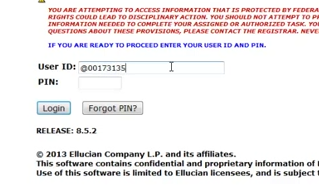
\includegraphics[scale=0.5]{images/login}
\item \textbf{Do you know where to go next?}

While it may not be the prettiest design, I have a pretty good grasp of the layout and where to go next depending on what I want to do.
\item \textbf{Does the product provide enough information for you to continue? Why? Why not?}

Yes, I would say it provides sufficient information for me to proceed, however I don\textquotesingle t think it would be a bad thing to add more descriptions of what each link does.  
\item \textbf{Does the product behave as expected?}

Yes, while it may not be the best design, the functionality seems to work fine, and from my own experiences with banner at W\&M I've never had issues with back end functionality.  
\item \textbf{Does the product assume knowledge that the user may not have?}

Not really.  Considering the targeted user is a college student, I don\textquotesingle t think the product is making any assumptions about the abilities of its users that it shouldn\textquotesingle t be.  
\item \textbf{Is information carried from one step of the task to the next?}

There are a few cases where information seems to be carried from one step to another.  The first and most obvious is when the user enters their student ID number.  From every screen after this the app remembers what student is logged in.  Also, the user can click a specific course and they are then taken to a new page showing all available sections of that course.  
\item \textbf{Does the product use language that the user will understand?}

Yes, the language used is appropriate for the service the product provides.  
\item \textbf{Do users understand whether the action they took has been completed?}

For the most part the product does a good job at giving the user success/error messages.  For example, when you register for a class, that class shows up in your queue of current courses.  Also, if you attempted to register and it was unsuccessful for some reason, the user is presented with a short message explaining why the action failed.  
\item \textbf{Make notes on every screen and consider how the journey feels. Is it short and smooth or 
long and complicated?}

The first few screens explaining how to get to the course registration part of the product seemed fairly straightforward and easy to follow.  On the page where the user is selecting a registration term, I can see how this might cause some confusion.  I\textquotesingle ve been using the process for quite some time but it may be unclear to a new user whether you should select the current term or the term you\textquotesingle ll be in when taking the classes.  While fairly intuitive to me, it also might not be obvious if you can select more than one option from the look up class subject drop down list.  Again, when actually performing the action of registering for a class, there is no explanation or warning for what will happen if you attempt to register for more than one class at a time.  This is the kind of thing that could lead to accidents down the line.  All in all, I think the main flaw in the banner course registration system are the aesthetics.  Something that is so commonly used among large institutions of higher learning should have a more attractive layout.  However, the functionality on the back end seems to be sound which is probably the priority in a product like this one.  

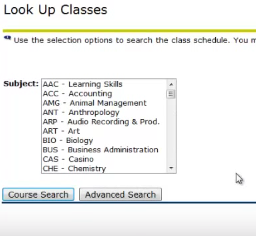
\includegraphics[scale=0.5]{images/subjects} 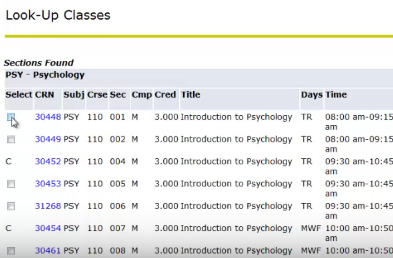
\includegraphics[scale=0.5]{images/register}
\end{enumerate}

\item Nielsen\textquotesingle s 10 Usability Heuristics
\begin{enumerate}[1)]
\item \textbf{Visibility of system status}

While concise, I do think the system gives adequate feedback based on what the user has entered.  That said, I don\textquotesingle t think it would be a bad thing to add more descriptions and such for the links on the site.  
\item \textbf{Match between system and the real world}

Since this app is aimed at college students, I think the language used in the app is an appropriate match between the system and the real world.  
\item \textbf{User control and freedom}

In the case of the user adding/dropping a class, the product is lacking in this area.  Once a class has been dropped, for example, there is no way to add it back except to go find the class listing or CRN number and re-add it.  At this point, another student might have snatched up that opening.  
\item \textbf{Consistency and standards}

The product seems to be pretty consistent in the language and standards it used to describe processes.  In this case, I don\textquotesingle t think any changes need to be made.  
\item \textbf{Error prevention}

The only case when this might be a concern is when a user tries to register for a class which overlaps with another on their schedule, or they don\textquotesingle t have the required prerequisites for.  However, I don\textquotesingle t think it\textquotesingle s really much trouble to display that error message after the request has been done instead of before.  A scenario where this could come into play is when the user attempts to register for more than one class and is successfull at one but not the other.  In this case, the product should be thorough in informing the user if it at least process half of their request, and if not, it should save the information they entered previously.  
\item \textbf{Recognition rather than recall}

This principle comes into play when the user registers for classes using CRN numbers.  I know that I personally often copy the CRN numbers of the classes I want into another document and then copy them into the text boxes when I want to register.  To me, this seems like an unnecessarily complicated process, and it should be accomplished more easily through a single click.  
\item \textbf{Flexibility and efficiency of use}

There do not seem to be any accelerators for this product.  For example, there should be easy access between the browse page and the register page.  As it appears now, you have to keep navigating through all the links in the page to get from one to the other, which can be a pain if you just want to check the availability of a class or what professor is teaching it.  
\item \textbf{Aesthetic and minimalist design}

There doesn\textquotesingle t appear to be too much irrelevant information but there are instances where information is redundant.  For example, there are tabs at the top of the page with links to different pages, but these links are duplicated in the list of options further down on the page.  
\item \textbf{Help users recognize, diagnose and recover from errors}

The product actually does a pretty good job of giving descriptive error messages.  For example, if you try to register for a class that you have a time conflict with, it gives you a message stating there was a conflict and which class it related to.  
\item \textbf{Help and documentation}

I\textquotesingle ve never actually needed to go to any help menus when using banner registration so I guess this is a good indicator that it\textquotesingle s not often needed, at least in my case.  However, there is a help tab at the top of the page, but when I click it it only directs me to phone numbers for administrative offices at the school.  
\end{enumerate}
\end{enumerate}
\end{document}




































